\begin{center}
    \large \textbf{1. Előadás}\\
    Bevezetés, anyagi pont kinematikája
\end{center}
\setstretch{1.5}
\underline{Elméleti összefoglaló:}
\begin{center}
    \Tree[.{\textbf{Dinamika}}
        [.{\textcolor{red}{\textbf{Kinematika}}\\A testek mozgásának leírásával foglalkozik}   
        ]
        [.{\textbf{Kinetika}\\Testek mozgásának okaival foglalkozik}
        ]
    ]
\end{center}
Mivel a bennünket körülvevő világ rendkívül összetett, közelítésekkel kell élnünk és a jelenség szempontjából fontosabb körülményeket kell kiemelnünk/figyelembe vennünk. Ezt hívjuk modellalkotásnak.\\\\
\textbf{Első modell:} Anyagi pont méretei lényegtelenek a vizsgált probléma szempontjából, tömegét viszont figyelembe vesszük a későbbiekben.\\
\textbf{Megjegyzés:} Ugyanazt a testet különböző feladatokban más-más mechanikai modellekkel vehetjük figyelembe.
\begin{tcolorbox}[colback=MidnightBlue!5!white,colframe=MidnightBlue!60!black,title= Példa]
Az úton közlekedő járműveket anyagi pontként modellezük, hogy a járműforgalomra vagyunk kiváncsiak, de hogyha a jármű manővereit is figyelembe akarjuk venni, akkor fontossá válik az autó alakja, tömegelosztása stb., így merev testként modellezük.
\end{tcolorbox}
\textbf{Alapvető fogalmak:}\\
Bármely anyagi test helyzete és mozgás más testekhez képest értelmezhető, tehát ki kell választanunk ezt a testet/testeket. Ezt vonatkoztatási rendszernek hívjuk. Ezt mindig meg kell adnunk, mert a mozgás különböző lehet más vonatkoztatási rendszerből nézve.
\begin{itemize}
    \item Gépkocsi gördülő kerekének egy pontja a karosszériához képest körpályán mozog az úthoz képest ciklois görbén.
    \item Mozgó járműben az utastér pontjait állónak látjuk és úgy tűnik, mintha a környezet mozogna
\end{itemize}  
A mozgások leírásához koordináta-rendszert kell felvennünk, ezt úgy célszerű felvenni, hogy a lehető legegyszerűbb legyen ebben a feladat megoldása.  
\begin{tcolorbox}[colback=MidnightBlue!5!white,colframe=MidnightBlue!60!black,title= Definíció]
\textbf{Mozgástörvény:} Az a függvény, mely egyértelműen megadja, hogy a vizsgált test pontjainak helye hogyan változik az időben. Anyagi pont esetében a mozgástörvény a helyvektor időbeli változását megadó vektorértékű \(\underline{r}(t)\) függvény.
$$\underline{r}(t) = \begin{bmatrix}
    x(t)\\
    y(t)\\
    z(t)
\end{bmatrix},$$
\begin{center}
    ahol \(x(t), y(t), z(t)\) skalárfüggvények.
\end{center}
ha ezeket együtt ábrázoljuk az idő koordinátáját elhagyva, akkor az anyagi pont pályáját kapjuk:
\begin{center}
\usetikzlibrary {3d}
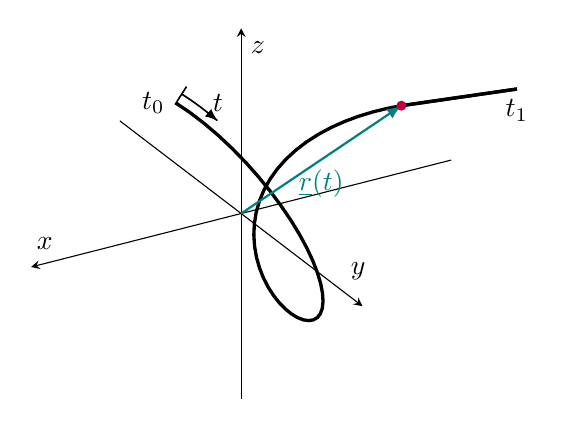
\begin{tikzpicture}[x=10cm,y=10cm]
    \begin{axis}[
        view={150}{30}, % Adjust the view angle
        axis lines=center,
        xlabel={$x$},
        ylabel={$y$},
        zlabel={$z$},
        xmin=-5, xmax=5,
        ymin=-1, ymax=1,
        zmin=-1, zmax=1,
        ticks=none, % Hide axis ticks
        width=10cm, % Adjust the width of the plot
        height=10cm, % Adjust the height of the plot
        enlargelimits=0.3, % Add some padding to the plot
    ]
    \def\param{-28}

    % Define the parametric equation for a one-loop helix
    \addplot3[
        domain=\param:10, % One loop corresponds to one full cycle (2*pi)
        samples=50, % Increase the number of samples for a smoother curve
        variable=t,
        samples y = 0,
        line width=1.2pt, % Adjust the line width
    ]({t/5}, {cos(10*t)}, {sin(8*t)});

    % Line segment
    \addplot3[
        domain=\param:-50,
        samples=50, % Increase the number of samples for a smoother curve
        variable=t,
        samples y = 0,
        line width=1.2pt, % Adjust the line width
    ]({t/5}, {cos(10*\param)}, {sin(8*\param) + (t/200) - \param/200});

    % Add the point
    \addplot3[mark options = {color=black,scale=0.8, color = purple},mark = *]
    coordinates {({\param/5},{cos(10*\param)}, {sin(8*\param)})};
    
    % Coordinates of the point
    \def\rx{\param/5}
    \def\ry{cos(10*\param)}
    \def\rz{sin(8*\param)}
    
    % r(t)
    \addplot3[line width=0.8pt, color = teal] coordinates {
        (0,0,0)
        ({\rx/2}, {\ry/2}, {\rz/2})
        } node[below, pos=1] {$\underline{r}(t)$};
\addplot3[-latex, line width=0.8pt, color = teal] coordinates {
        ({\rx/2}, {\ry/2}, {\rz/2})
        ({\rx}, {\ry}, {\rz})};

    %t_0
    \addplot3[
        domain=9.9:10,
        samples=50, % Increase the number of samples for a smoother curve
        variable=t,
        samples y = 0,
        line width=1.2pt, % Adjust the line width
    ]({t/5}, {cos(10*t)}, {sin(8*t)}) node[left,pos=1] {$t_0$};

    %t_1
    \addplot3[
        domain=\param:-50,
        samples=50, % Increase the number of samples for a smoother curve
        variable=t,
        samples y = 0,
        line width=1.2pt, % Adjust the line width
    ]({t/5}, {cos(10*\param)}, {sin(8*\param) + (t/200) - \param/200}) node[below,pos=1] {$t_1$};

    %t |-->
    \addplot3[
        domain=10:8,
        samples=50, % Increase the number of samples for a smoother curve
        variable=t,
        samples y = 0,
        |-latex,
        line width=0.6pt % Adjust the line width
    ]({t/5 - 0.5}, {cos(10*t) - 0.1}, {sin(8*t)}) node[above, pos=1] {$t$};

    \end{axis}
    \end{tikzpicture}
\end{center}
\end{tcolorbox}
\begin{tcolorbox}[colback=MidnightBlue!5!white,colframe=MidnightBlue!60!black,title= Definíció]
\textbf{Pálya:} Az anyagi pont helyvektorának grafikonja térben (időfüggés nélkül)\\
\textbf{Anyagi pont pillanyatni sebessége:} az \(\underline{r}(t)\) helyvektor idő szerinti deriváltja
$$\underline{v}(t) = \dfrac{d \underline{r}(t)}{dt} = \underline{r}(t)$$
\underline{\underline{Fontos}} csak akkor nulla egy vektor időszerinti deriváltja, ha sem a mozgása sem az iránya nem változik!
\end{tcolorbox}

\begin{tcolorbox}[colback=MidnightBlue!5!white,colframe=MidnightBlue!60!black,title= Definíció]
\textbf{Anyagi pont pillanatnyi gyorsulása:} az \(\underline{r}(t)\) sebességvektor idő szerinti deriváltja
$$\underline{a}(t) = \dfrac{d^2r(t)}{dt^2} = \underline{\dot{v}}(t) = \ddot{\underline{r}}(t)$$
Csak az egyenes vonalú, egyenletes mozgás esetén nulla a gyorsulás!
\begin{multicols}{2}
    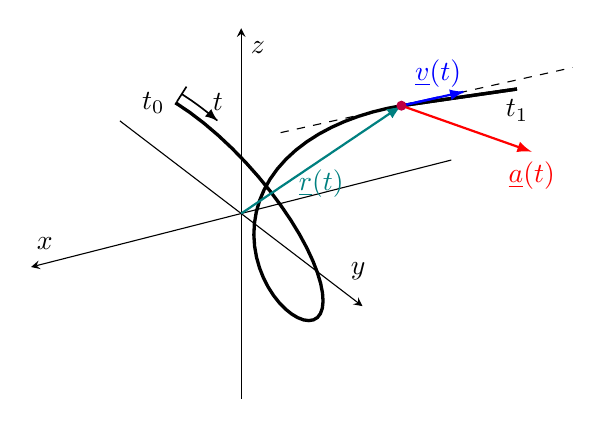
\begin{tikzpicture}[x=10cm,y=10cm]
        \begin{axis}[
            view={150}{30}, % Adjust the view angle
            axis lines=center,
            xlabel={$x$},
            ylabel={$y$},
            zlabel={$z$},
            xmin=-5, xmax=5,
            ymin=-1, ymax=1,
            zmin=-1, zmax=1,
            ticks=none, % Hide axis ticks
            width=10cm, % Adjust the width of the plot
            height=10cm, % Adjust the height of the plot
            enlargelimits=0.3, % Add some padding to the plot
        ]
        \def\param{-28}
    
        % Define the parametric equation for a one-loop helix
        \addplot3[
            domain=\param:10, % One loop corresponds to one full cycle (2*pi)
            samples=50, % Increase the number of samples for a smoother curve
            variable=t,
            samples y = 0,
            line width=1.2pt, % Adjust the line width
        ]({t/5}, {cos(10*t)}, {sin(8*t)});
    
        % Line segment
        \addplot3[
            domain=\param:-50,
            samples=50, % Increase the number of samples for a smoother curve
            variable=t,
            samples y = 0,
            line width=1.2pt, % Adjust the line width
        ]({t/5}, {cos(10*\param)}, {sin(8*\param) + (t/200) - \param/200});
    
        % Coordinates of the point
        \def\rx{\param/5}
        \def\ry{cos(10*\param)}
        \def\rz{sin(8*\param)}

        % Add the point
        \addplot3[mark options = {color=black,scale=0.8, color = purple},mark = *]
                coordinates {({\rx}, {\ry}, {\rz})};
        

        % r(t)
        \addplot3[line width=0.8pt, color = teal] coordinates {
                (0,0,0)
                ({\rx/2}, {\ry/2}, {\rz/2})
                } node[below, pos=1] {$\underline{r}(t)$};
        \addplot3[-latex, line width=0.8pt, color = teal] coordinates {
                ({\rx/2}, {\ry/2}, {\rz/2})
                ({\rx}, {\ry}, {\rz})};
    
        %t_0
        \addplot3[
            domain=9.9:10,
            samples=50, % Increase the number of samples for a smoother curve
            variable=t,
            samples y = 0,
            line width=1.2pt, % Adjust the line width
        ]({t/5}, {cos(10*t)}, {sin(8*t)}) node[left,pos=1] {$t_0$};
    
        %t_1
        \addplot3[
            domain=\param:-50,
            samples=50, % Increase the number of samples for a smoother curve
            variable=t,
            samples y = 0,
            line width=1.2pt, % Adjust the line width
        ]({t/5}, {cos(10*\param)}, {sin(8*\param) + (t/200) - \param/200}) node[below,pos=1] {$t_1$};
    
        %t |-->
        \addplot3[
            domain=10:8,
            samples=50, % Increase the number of samples for a smoother curve
            variable=t,
            samples y = 0,
            |-latex,
            line width=0.6pt % Adjust the line width
        ]({t/5 - 0.5}, {cos(10*t) - 0.1}, {sin(8*t)}) node[above, pos=1] {$t$};

        %tangent line to point r
        \addplot3[
            dashed,
            domain=-5:-70,
            samples=50, % Increase the number of samples for a smoother curve
            variable=t,
            samples y = 0,
            line width=0.4pt, % Adjust the line width
        ]({t/5}, {cos(10*\param)}, {sin(8*\param) + (t)/700 - \param/700});

        %v(t)
        \addplot3[
            domain=\param:-35,
            samples=50, % Increase the number of samples for a smoother curve
            variable=t,
            samples y = 0,
            line width=0.8pt, % Adjust the line width
            color = blue,
        ]({t/5}, {cos(10*\param)}, {sin(8*\param) + (t)/700 - \param/700}) node[above, pos=1] {$\underline{v}(t)$};
        \addplot3[
            domain=\param:-40,
            samples=50, % Increase the number of samples for a smoother curve
            variable=t,
            samples y = 0,
            line width=0.8pt, % Adjust the line width
            color = blue,
            -latex,
        ]({t/5}, {cos(10*\param)}, {sin(8*\param) + (t)/700 - \param/700});

        %a(t)
        \addplot3[
            domain=\param:-45,
            samples=50, % Increase the number of samples for a smoother curve
            line width=0.8pt, % Adjust the line width
            color = red,
            -latex,
        ] coordinates {
            ({\rx}, {\ry}, {\rz})    
            ({\rx -2}, 1.2, {\rz})} node[below, pos=1] {$\underline{a}(t)$};
    
        \end{axis}
        \end{tikzpicture}
    \columnbreak

    A sebesség vektor párhuzamos a pálya érintőjével!
    A gyorsulásvektor is megadható két természetes komponens segítségével, melyek közül az egyik a sebesség nagyságának változásával kapcsolatos és érintőirányú, a másik a sebesség irányának változását jellemzi és az előzőre merőleges.
\end{multicols}
\end{tcolorbox}

Vagyis a
\begin{itemize}
    \item tangenciális gyorsulás: \(\underline{a}_t = a_t \cdot \underline{e}_t\), ahol \(\underline{e}_t \mid\mid \underline{v}\) és \(\underline{e}_t\) egy bázisvektor
    \item normális gyorsulás: \(\underline{a}_n = a_n \cdot \underline{e}_n\), ahol \(\underline{e}_t \bot  \underline{e}_n\) és \(\underline{a}_n = \underline{a} - \underline{a}_t\)
\end{itemize}
$$\underline{e}_n = \dfrac{\underline{a}_n}{a_n} \equiv \dfrac{\underline{a}_n}{\mid \underline{a}_n \mid} $$
Ezzel:
\begin{center}
    \fbox{\(\underline{a} = a_t\cdot \underline{e}_t + a_n\cdot \underline{e}_n\)}
\end{center}
Megkülönböztetünk még egy irányt, a binormális irányt, mely az előző kettőre merőleges
$$\underline{e}_b = \underline{e}_t \times  \underline{e}_n$$
\textbf{Tangenciális gyorsulás:} \(a_t = \mid \underline{\dot{v}} \mid \)\\
\textbf{Normális gyorsulás:} \(a_n = \dfrac{v^2}{\varrho}\), ahol a \(\varrho\) a görbületi sugár
\newpage
\begin{multicols}{2}
    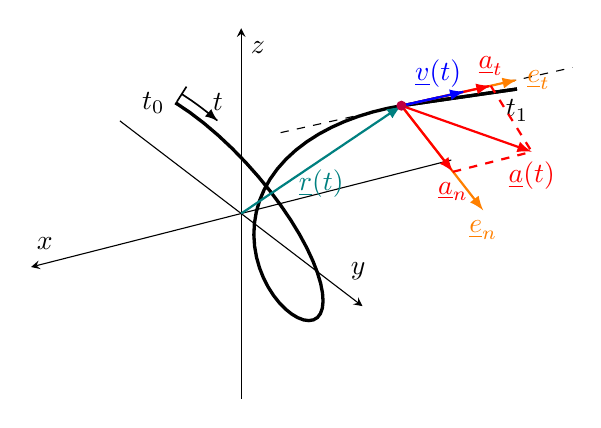
\begin{tikzpicture}
        \begin{axis}[
            view={150}{30}, % Adjust the view angle
            axis lines=center,
            xlabel={$x$},
            ylabel={$y$},
            zlabel={$z$},
            xmin=-5, xmax=5,
            ymin=-1, ymax=1,
            zmin=-1, zmax=1,
            ticks=none, % Hide axis ticks
            width=10cm, % Adjust the width of the plot
            height=10cm, % Adjust the height of the plot
            enlargelimits=0.3, % Add some padding to the plot
        ]
        \def\param{-28}
    
        % Define the parametric equation for a one-loop helix
        \addplot3[
            domain=\param:10, % One loop corresponds to one full cycle (2*pi)
            samples=50, % Increase the number of samples for a smoother curve
            variable=t,
            samples y = 0,
            line width=1.2pt, % Adjust the line width
        ]({t/5}, {cos(10*t)}, {sin(8*t)});
    
        % Line segment
        \addplot3[
            domain=\param:-50,
            samples=50, % Increase the number of samples for a smoother curve
            variable=t,
            samples y = 0,
            line width=1.2pt, % Adjust the line width
        ]({t/5}, {cos(10*\param)}, {sin(8*\param) + (t/200) - \param/200});
    
        % Coordinates of the point
        \def\rx{\param/5}
        \def\ry{cos(10*\param)}
        \def\rz{sin(8*\param)}

        % Add the point
        \addplot3[mark options = {color=black,scale=0.8, color = purple},mark = *]
                coordinates {({\rx}, {\ry}, {\rz})};
        

        % r(t)
        \addplot3[line width=0.8pt, color = teal] coordinates {
                (0,0,0)
                ({\rx/2}, {\ry/2}, {\rz/2})
                } node[below, pos=1] {$\underline{r}(t)$};
        \addplot3[-latex, line width=0.8pt, color = teal] coordinates {
                ({\rx/2}, {\ry/2}, {\rz/2})
                ({\rx}, {\ry}, {\rz})};
    
        %t_0
        \addplot3[
            domain=9.9:10,
            samples=50, % Increase the number of samples for a smoother curve
            variable=t,
            samples y = 0,
            line width=1.2pt, % Adjust the line width
        ]({t/5}, {cos(10*t)}, {sin(8*t)}) node[left,pos=1] {$t_0$};
    
        %t_1
        \addplot3[
            domain=\param:-50,
            samples=50, % Increase the number of samples for a smoother curve
            variable=t,
            samples y = 0,
            line width=1.2pt, % Adjust the line width
        ]({t/5}, {cos(10*\param)}, {sin(8*\param) + (t/200) - \param/200}) node[below,pos=1] {$t_1$};
    
        %t |-->
        \addplot3[
            domain=10:8,
            samples=50, % Increase the number of samples for a smoother curve
            variable=t,
            samples y = 0,
            |-latex,
            line width=0.6pt % Adjust the line width
        ]({t/5 - 0.5}, {cos(10*t) - 0.1}, {sin(8*t)}) node[above, pos=1] {$t$};

        %tangent line to point r
        \addplot3[
            dashed,
            domain=-5:-70,
            samples=50, % Increase the number of samples for a smoother curve
            variable=t,
            samples y = 0,
            line width=0.4pt, % Adjust the line width
        ]({t/5}, {cos(10*\param)}, {sin(8*\param) + (t)/700 - \param/700});

        %e_t
        \addplot3[
            domain=\param:-50,
            samples=50, % Increase the number of samples for a smoother curve
            variable=t,
            samples y = 0,
            line width=0.8pt, % Adjust the line width
            color = orange,
            -latex,
        ]({t/5}, {cos(10*\param)}, {sin(8*\param) + (t)/700 - \param/700}) node[right, pos=1] {$\underline{e}_t$};

        %a_t
        \addplot3[
            domain=\param:-45,
            samples=50, % Increase the number of samples for a smoother curve
            variable=t,
            samples y = 0,
            line width=0.8pt, % Adjust the line width
            color = red,
            -latex,
        ]({t/5}, {cos(10*\param)}, {sin(8*\param) + (t)/700 - \param/700}) node[above, pos=1] {$\underline{a}_t$};

        %v(t)
        \addplot3[
            domain=\param:-35,
            samples=50, % Increase the number of samples for a smoother curve
            variable=t,
            samples y = 0,
            line width=0.8pt, % Adjust the line width
            color = blue,
        ]({t/5}, {cos(10*\param)}, {sin(8*\param) + (t)/700 - \param/700}) node[above, pos=1] {$\underline{v}(t)$};
        \addplot3[
            domain=\param:-40,
            samples=50, % Increase the number of samples for a smoother curve
            variable=t,
            samples y = 0,
            line width=0.8pt, % Adjust the line width
            color = blue,
            -latex,
        ]({t/5}, {cos(10*\param)}, {sin(8*\param) + (t)/700 - \param/700});

        %a(t)
        \addplot3[
            domain=\param:-45,
            samples=50, % Increase the number of samples for a smoother curve
            line width=0.8pt, % Adjust the line width
            color = red,
            -latex,
        ] coordinates {
            ({\rx}, {\ry}, {\rz})    
            ({\rx -2}, 1.2, {\rz})} node[below, pos=1] {$\underline{a}(t)$};

        %a_t -- a(t)
        \addplot3[
            domain=\param:-45,
            samples=50, % Increase the number of samples for a smoother curve
            line width=0.8pt, % Adjust the line width
            color = red,
            dashed,
        ] coordinates {
            ({-45/5}, {cos(10*\param)}, {sin(8*\param) + (-45)/700 - \param/700})    
            ({\rx -2}, 1.2, {\rz})};
            
        %e_n
        \addplot3[
            domain=\param:-45,
            samples=50, % Increase the number of samples for a smoother curve
            line width=0.8pt, % Adjust the line width
            color = orange,
            -latex,
        ] coordinates {
            ({\rx}, {\ry}, {\rz})    
            ({\rx + 1.58}, 1.8, {\rz})} node[below, pos=1] {$\underline{e}_n$};
        
        %a_n
        \addplot3[
            domain=\param:-45,
            samples=50, % Increase the number of samples for a smoother curve
            line width=0.8pt, % Adjust the line width
            color = red,
            -latex,
        ] coordinates {
            ({\rx}, {\ry}, {\rz})    
            ({\rx + 1}, 1.2, {\rz})} node[below, pos=1] {$\underline{a}_n$};


        %a_n -- a(t)
        \addplot3[
            domain=\param:-45,
            samples=50, % Increase the number of samples for a smoother curve
            line width=0.8pt, % Adjust the line width
            color = red,
            dashed,
        ] coordinates {
            ({\rx + 1}, 1.2, {\rz})    
            ({\rx -2}, 1.2, {\rz})};
    
        \end{axis}
        \end{tikzpicture}
    \columnbreak

    A pálya, akkor lehet igazi térbeli görbe, ha a mozgás során folyamatosan változó irányú \(\underline{e}_t\) és \(\underline{e}_n\) vektorok által kifeszített sík (simulósík) helyzete változik. (A simulósík pálya menti elfordulását a tartozó \(\underline{\dddot{r}}(t)\) (jerk) jellemzi)
\end{multicols}
\begin{tcolorbox}[colback=MidnightBlue!5!white,colframe=MidnightBlue!60!black,title= Definíció]
\textbf{Jerk:} Kinetikai egyenleteknél nem használatos, de például tömegközlekedésnél a testtartásunk megváltoztatásával könnyen alkalmazkodunk a gyorsuláshoz, de ennek megváltozásához viszont nem.
\end{tcolorbox}
 \textbf{Pályához illeszkedő koordináták:}
\begin{itemize}
    \item A sebesség előjeles nagysága a pályasebesség
    \item A pályasebesség további deriválásával a gyorsulás érintő irányú kompenensének az előjeles nagyságát kapjuk, ez a pályagyorsulás.
    \item Értelmezzük még keringési szögsebességet és szöggyorsulást, de fontos megjegyezni, hogy anyagi pontnak nincs szögsebesség vagy szöggyorsulása! (A szögsebesség az elfordulás ütemét jelenti!)
\end{itemize}
\begin{tcolorbox}[colback=MidnightBlue!5!white,colframe=MidnightBlue!60!black,title= Definíció]
Az adott pályán mozgó anyagi pont pozícióját egyértelműen megadhatjuk egy választott kezdőpontból mért \(s\) ívhosszparaméterrel, azaz a pálya mentén mért koordinátával. Az ívhossz paraméter időbeli változása \(s(t)\) a befutási törvény.
\begin{multicols}{2}
    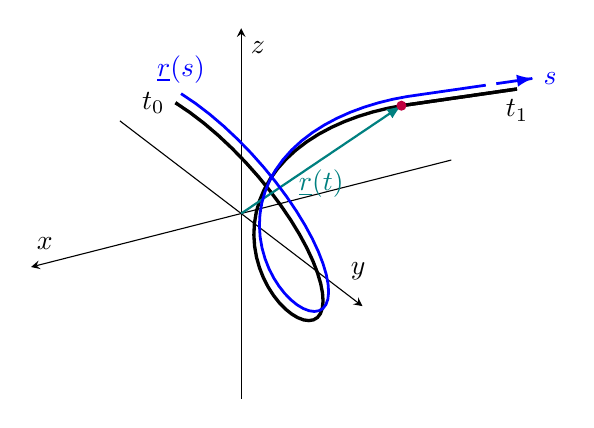
\begin{tikzpicture}
        \begin{axis}[
            view={150}{30}, % Adjust the view angle
            axis lines=center,
            xlabel={$x$},
            ylabel={$y$},
            zlabel={$z$},
            xmin=-5, xmax=5,
            ymin=-1, ymax=1,
            zmin=-1, zmax=1,
            ticks=none, % Hide axis ticks
            width=10cm, % Adjust the width of the plot
            height=10cm, % Adjust the height of the plot
            enlargelimits=0.3, % Add some padding to the plot
        ]
        \def\param{-28}
    
        % Define the parametric equation for a one-loop helix
        \addplot3[
            domain=\param:10, % One loop corresponds to one full cycle (2*pi)
            samples=50, % Increase the number of samples for a smoother curve
            variable=t,
            samples y = 0,
            line width=1.2pt, % Adjust the line width
        ]({t/5}, {cos(10*t)}, {sin(8*t)});
    
        % Line segment
        \addplot3[
            domain=\param:-50,
            samples=50, % Increase the number of samples for a smoother curve
            variable=t,
            samples y = 0,
            line width=1.2pt, % Adjust the line width
        ]({t/5}, {cos(10*\param)}, {sin(8*\param) + (t/200) - \param/200});
    
        % Coordinates of the point
        \def\rx{\param/5}
        \def\ry{cos(10*\param)}
        \def\rz{sin(8*\param)}

        % Add the point
        \addplot3[mark options = {color=black,scale=0.8, color = purple},mark = *]
                coordinates {({\rx}, {\ry}, {\rz})};
        

        % r(t)
        \addplot3[line width=0.8pt, color = teal] coordinates {
                (0,0,0)
                ({\rx/2}, {\ry/2}, {\rz/2})
                } node[below, pos=1] {$\underline{r}(t)$};
        \addplot3[-latex, line width=0.8pt, color = teal] coordinates {
                ({\rx/2}, {\ry/2}, {\rz/2})
                ({\rx}, {\ry}, {\rz})};
    
        %t_0
        \addplot3[
            domain=9.9:10,
            samples=50, % Increase the number of samples for a smoother curve
            variable=t,
            samples y = 0,
            line width=1.2pt, % Adjust the line width
        ]({t/5}, {cos(10*t)}, {sin(8*t)}) node[left,pos=1] {$t_0$};
    
        %t_1
        \addplot3[
            domain=\param:-50,
            samples=50, % Increase the number of samples for a smoother curve
            variable=t,
            samples y = 0,
            line width=1.2pt, % Adjust the line width
        ]({t/5}, {cos(10*\param)}, {sin(8*\param) + (t/200) - \param/200}) node[below,pos=1] {$t_1$};

        %r(s)
        \addplot3[
            domain=\param:10, % One loop corresponds to one full cycle (2*pi)
            samples=50, % Increase the number of samples for a smoother curve
            variable=t,
            samples y = 0,
            line width=1pt, % Adjust the line width
            color = blue,
        ]({t/5 - 0.5}, {cos(10*t)-0.1}, {sin(8*t)}) node[above, pos=1]{$\underline{r}(s)$};
        \addplot3[
            domain=\param:-43,
            samples=50, % Increase the number of samples for a smoother curve
            variable=t,
            samples y = 0,
            line width=1pt, % Adjust the line width
            color = blue,
        ]({t/5 - 0.5}, {cos(10*\param)-0.1}, {sin(8*\param) + (t/200) - \param/200});

        %s
        \addplot3[
            domain=-45:-52,
            samples=50, % Increase the number of samples for a smoother curve
            variable=t,
            samples y = 0,
            line width=1pt, % Adjust the line width
            -latex,
            color = blue,
        ]({t/5 - 0.5}, {cos(10*\param)-0.1}, {sin(8*\param) + (t/200) - \param/200}) node[right, pos=1]{$s$};

        \end{axis}
        \end{tikzpicture}
    \columnbreak

  Pályasebesség: \(v=\dot{s}(t)\)\\
  Pályagyorsulás: \(a = \ddot{s}(t)\)\\
  Ezeket együttesen \underline{foronómiai görbéknek} hívjuk!
\end{multicols}
\end{tcolorbox}
\newpage
\textbf{Kényszerek:}
\begin{tcolorbox}[colback=MidnightBlue!5!white,colframe=MidnightBlue!60!black,title= Definíció]
    \textbf{Szabadsági fok (DoF):} Azon független skalár függvények száma, melyek egyértelműen megadják a rendszer mozgástörvényét!
    \end{tcolorbox}
\begin{tcolorbox}[colback=MidnightBlue!5!white,colframe=MidnightBlue!60!black,title= Definíció]
    Kényszernek előírt geometriai vagy kinematikai feltételek melyek korlátozásokat jelentenek a mozgásokra nézve.\\
    \textbf{Osztályozásuk:}
    \begin{itemize}
        \begin{multicols}{2}
        \item holonóm (geometriai)
        \item anholonóm (kinematikai)
        
        \columnbreak
        \item szkleronóm (időtől független)
        \item reanóm (időtől függő)
        \end{multicols}
    \end{itemize}
\end{tcolorbox}
\newpage
\begin{center}
    \large \textbf{1. Gyakorlat}\\
    Pont mozgása egyenes és körpályán, foronómiai görbék
\end{center}
\begin{tcolorbox}[colback=MidnightBlue!5!white,colframe=MidnightBlue!60!black,title= 1. Feladat]
\setstretch{1.2}
    \textbf{Adatok:}
\begin{center}
    \begin{multicols}{3}
        \(R = 0,3\ m\)

        \columnbreak

        \(\underline{v}_s =\) állandó

        \columnbreak

        \(v_s = 5\ ms^{-1}\)
    \end{multicols}
\end{center}
\textbf{Feladatok:}
\begin{itemize}
    \item Határozza meg a \(P\) pont sebességét a $\varphi$ paraméter függvényében!
    \item Határozza meg a \(P\) pont gyorsulását hasonlóképpen!
    \item Számítsa ki a \(\varphi_1 = 75^{\circ}\)-hoz tartozó \(\underline{a}_1\) és \(\underline{v}_1\) a gyorsulást, illetve sebességét!
    \item Számítsa ki és ábrázolja az \(\underline{a}_1\) gyorsulás normális és tangenciális komponens
    \item A \(\varphi_1 = 75^{\circ}\) szöghelyzetben számítsa ki a páya \(\varrho_1\) görbületi sugarát!
\end{itemize}
\Pointilles{22}
\end{tcolorbox}
\begin{tcolorbox}[colback=MidnightBlue!5!white,colframe=MidnightBlue!60!black,title= 1. Feladat]
    \setstretch{1.2}
    \Pointilles{38}
\end{tcolorbox}